\documentclass[12pt,a4paper]{article}
\usepackage[utf8]{inputenc}
\usepackage[brazil]{babel}
\usepackage[T1]{fontenc}
\usepackage{graphicx}
\usepackage[alf]{abntcite}

\usepackage{times}

\title{Exercícios Sistemas Operacionais II \\ 
	Gerencia de Memória}
\author{Universidade Estadual do Centro-Oeste (UNICENTRO)\\
        Departamento de Ciência da Computação (DECOMP)\\
        Sistemas Operacionais II \\
        Professor Diego Marczal \\
	Paulo R. Urio \\ 
	Eduardo T. Feliczaki }

\newcommand{\pergunta}[1]{\vspace{10pt} \noindent \textbf{#1} \vspace{5pt}}

\begin{document}

\maketitle

\pergunta{1. Quais as funções básicas da gerência de memória?}

A função básica do gerenciador de memória é alocar dinamicamente porções
de memória para programas, quando requisitadas, e liberar para reuso 
quando não for mais necessária \cite{IBMMemoryManagement}.  Também deve
gerenciar toda a memória disponível (memória principal e secundária) de 
forma transparente aos programas do \textsl{userspace} 
\cite{TheLinuxKernel}.


\pergunta{2. Considere um sistema computacional com 40Kb de memória principal e 
que utilize um sistema operacional de 10Kb que implemente alocação contígua de 
memória. Qual a taxa de subutilização da memória principal para um programa que 
ocupe 20Kb de memória?}

10 KB.


\pergunta{3. Suponha um sistema computacional com 64KB de memória principal e que utilize um
sistema operacional de 14KB que implemente alocação contígua de memória. Considere também
um programa de 80KB, formado por um módulo principal de 20KB e três módulos
independentes, cada um com 10KB,20KB e 30KB. Como o programa poderia ser executado
utilizando-se apenas a técnica de overlay?}

O sistema operacional será alocado no início da memória principal, deixando
50 KB para programas em \textsl{userspace} utilizarem.  \textsl{Overlay} é o 
processo de transferir um bloco de código de programa ou dados para a memória interna,
substituindo pelo bloco atual \cite{OxfordDictionary}.  Os blocos independentes
serão colocados na memória, no espaço dedicado ao \textsl{overlay}, um por vez 
para serem utilizados.  A memória
ficará organizada de acordo com a Figura \ref{OverlayPDF}.  O módulo principal
é encarregado de executar os \textsl{overlays}.

\begin{figure}[!ht]
  \centering
	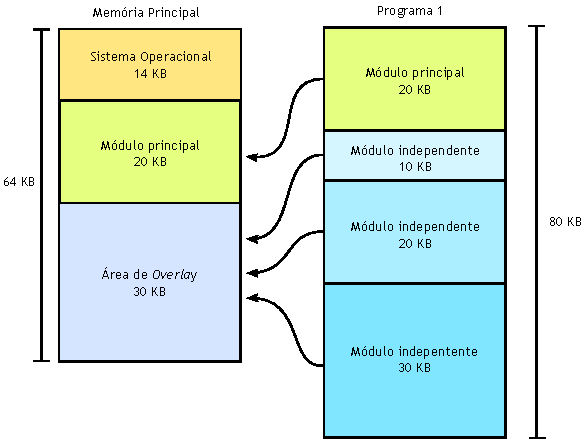
\includegraphics[scale=1]{img/overlay.pdf}
  \caption{Estado da memória principal \label{OverlayPDF}}
\end{figure}


\pergunta{4. Considerando o exercício anterior, se o módulo de 30KB tivesse seu 
tamanho aumentado para 40KB, seria possível executar o programa? Caso não possa, 
como o problema poderia ser contornado?}

Não seria possível executar o programa. Para se resolver o problema, o módulo
de 40KB deveria que ser quebrado em dois módulos indepententes para assim poder 
ser executado.  Ao tentar executar \textsl{overlay} no módulo independente de
40 KB em uma área de \textsl{overlay} de 30KB, ocorre a fragmentação 
externa \cite{ContiguousTechniques}.


\pergunta{5. Qual a diferença entre fragmentação interna e externa da memória 
principal?}

A fragmentação interna ocorre quando os programas não preenchem as partições
onde são carregados, ocorre nos sistemas de alocação absoluta e nos sistemas
de alocação relocável.
A fragmentação externa ocorre nos sistemas de alocação dinâmica ocorre quando
programas são terminados mas não são completamente liberados da memória, deixando
cada vez espaços menores na memória, assim novos programas não podem ser executados.\\

\pergunta{6. Suponha um sistema computacional com 128KB de memória principal e que utilize um
sistema operacional de 64KB que implementa alocação particionada estática relocável.
Considere também que o sistema foi inicializado com três partições: P1 (8KB), P2 (24KB) e P3
(32KB). Calcule a fragmentação interna da memória principal após a carga de três programas:
PA, PB e PC.}

\pergunta{a) P1 $\leftarrow$ PA (6KB); P2 $\leftarrow$ PB (20KB); P3 $\leftarrow$ PC (28KB)}

\pergunta{b) P1 $\leftarrow$ PA (4KB); P2 $\leftarrow$ PB (16KB); P3 $\leftarrow$ PC (26KB)}

\pergunta{c) P1 $\leftarrow$ PA (8KB); P2 $\leftarrow$ PB (24KB); P3 $\leftarrow$ PC (32KB)}


\pergunta{7. Considerando o exercício anterior, seria possível executar quatro 
programas concorrentemente utlizando apenas a técnica de alocação particionada 
estática relocável? Se for possível, como? Considerando ainda o mesmo exercício, 
seria possível executar um programa de 36KB? Se for possível como?}


\pergunta{8. Qual a limitação da alocação particionada estática absoluta em relação a alocação estática
relocável?}



\pergunta{9. Considere que os processos da tabela a seguir estão aguardando para
serem executados e que cada um permanecerá na memória durante o tempo especificado. 
O sistema operacional ocupa uma área de 20Kb no início da memória e gerencia a 
memória utilizando um algoritmo de particionamento dinâmico modificado. 
A memória total disponível no sistema é de 64Kb e é alocada em blocos múltiplos 
de 4Kb.Os processos são alocados de acordo com sua identificação (em ordem crescente) 
e irão aguardar até obter a memória que necessitam. Calcule a perda de
memória por fragmentação interna e externa sempre que um processo é colocado ou 
retirado da memória. O sistema operacional compacta a memória apenas quando existem 
duas ou mais partições livres adjacentes.}

Processo Memória Tempo\\
1 30KB 5\\
2 6KB 10\\
3 36KB 5\\

	

\pergunta{10. Considerando as estratégias para escolha da partição dinamicamente, conceitue as estratégias
best-fit eworst-fit especificando prós e contras de cada uma.}


\pergunta{11. Considere um sistema que possua as seguintes área livres na memória principal,
ordenadascrescentemente: 10Kb, 4Kb, 20Kb, 18Kb, 7Kb, 9Kb, 12Kb e 15Kb. Para cada
programa abaixo, qualseria a partição alocada utilizando-se as estratégias first-fit, best-fit e
worst-fit (Tanenbaum, 1992)?}

\pergunta{a) 12KB}

First-Fit: 20 Kb\\
Best-Fit: 12 Kb\\
Worst-Fit: 20 Kb\\

\pergunta{b) 10KB}

First-Fit: 10 Kb\\
Best-Fit: 10 Kb\\
Worst-Fit: 20 Kb\\

\pergunta{c) 9KB}

First-Fit: 10 Kb\\
Best-Fit: 9 Kb\\
Worst-Fit: 20 Kb\\



\bibliography{main}

\end{document}

